\documentclass[letterpaper,11pt]{article}
\usepackage{graphicx}
\usepackage{listings}
\usepackage[super]{nth}
\usepackage[hyphens]{url}
\usepackage{hyperref}
\usepackage{amsmath}
\usepackage[makeroom]{cancel}
\usepackage[table]{xcolor}
\usepackage{comment}
\usepackage[space]{grffile}
\usepackage{csvsimple}
\usepackage{longtable}
\usepackage{adjustbox}


\newcommand*{\srcPath}{../src}%

\lstset{
	basicstyle=\footnotesize,
	breaklines=true,
}

\begin{document}

\begin{titlepage}

\begin{center}

\Huge{Assignment 2}

\Large{CS 734:  Introduction to Information Retrieval}

\Large{Fall 2017}

\Large{Grant Atkins}

\Large Finished on \today

\end{center}

\end{titlepage}

\newpage


% =================================
% First question
% =================================
\section*{1}

\subsection*{Question}

\begin{verbatim}
4.1. Plot rank-frequency curves (using a log-log graph) for 
words and bigrams in the Wikipedia collection available through 
the book website (http://www.searchengines-book.com). Plot a 
curve for the combination of the two. What are the best 
values for the parameter c for each curve?
\end{verbatim}

\subsection*{Answer}

For this question I wrote two files of code, \textbf{rankFreq.py} and \textbf{rankFreq.R} in with the ``small'' wiki dataset provided from the textbooks website . 
The first python file iterates through all of the wiki html files, tokenizes them, finds token frequency, and then writes them to a CSV in descending frequency order.
To retrieve the text from each of the html files I used Beautifulsoup. 
It should be noted when retrieving each token from the html files I did not take into account uppercase or lowercase as same terms, I treated them as different and more than probably affected the outcome of this answer.
After the code tokenizing the terms it created a list of unigrams and bigrams for all the terms keeping them in separate lists to count frequencies.
I used the NLTK python library to make bigram pairs.
The code for this is shown below in Listing \ref{lst:q1py}.
The top 10, ranked by token frequency, results are shown below in Figures \ref{fig:q1uni} and \ref{fig:q1bi}.
The full CSV files can be found in my Github repository \cite{github}.
Without removing stop words its apparent that words like ``the'' and ``of'' would some of the top unigram and bigram pairs.

 \lstinputlisting[frame=single,caption={Python script to tokenize and find frequencies and calculate C parameters},label=lst:q1py,captionpos=b,numbers=left,showspaces=false,showstringspaces=false,basicstyle=\footnotesize]{\srcPath/rankFreq.py}
 
 To create the graphs I used R's ggplot2 library. 
 The code to create these graphs is shown in Listing \ref{lst:q1R}.
 The figures created from the afore mentioned code are shown in Figure \ref{fig:q1p1}, \ref{fig:q1p2}, and \ref{fig:q1p3}.
For unigrams the best \textit{C} parameter was 0.14, while for bigrams it was 0.1.
 
  \lstinputlisting[frame=single,caption={Python script to tokenize and find frequencies and calculate C parameters},label=lst:q1R,captionpos=b,numbers=left,showspaces=false,showstringspaces=false,basicstyle=\footnotesize]{\srcPath/rankFreq.R}

%Finally when completing Enterprise search it should be noted that I don't have access to an intranet but I do have access to my own personal machine to conduct searches on my own file system.
%I used my operating system's implemented search in it file system and I also use the terminal command \textit{grep} to show a customized search on a subset of directories.
%Using my operating systems \textit{finder} program it searches across my entire computer of files with the words ``cs834-f17'' as shown in Figure \ref{fig:esearch1}. This type of seems more relatable to web search as it seem to generalize the results showing files that mention this term, but not every single file in my filesystem.
%When I used the \textit{grep} command searching any directories starting with ``cs'' it showed every occurrence where ``cs834-f17'' was used. This is more relatable to site search because it listed all locations of occurrence in these directories.

  \begin{figure}[h]
  \centering
  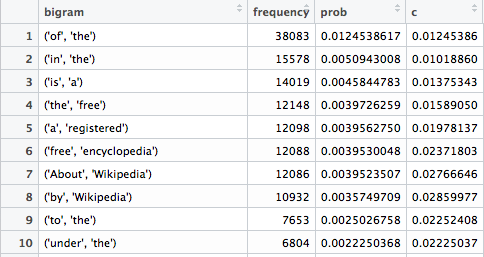
\includegraphics[scale=0.6]{unigram_10.png}
  \caption{Top 10 unigrams found}
  \label{fig:q1uni}
  \end{figure}

  \begin{figure}[h]
  \centering
  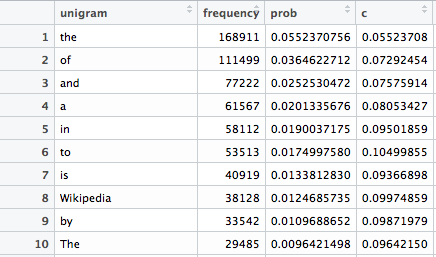
\includegraphics[scale=0.6]{bigram_10.png}
  \caption{Top 10 bigrams found}
  \label{fig:q1bi}
  \end{figure}
  
   \begin{figure}[h]
  \centering
  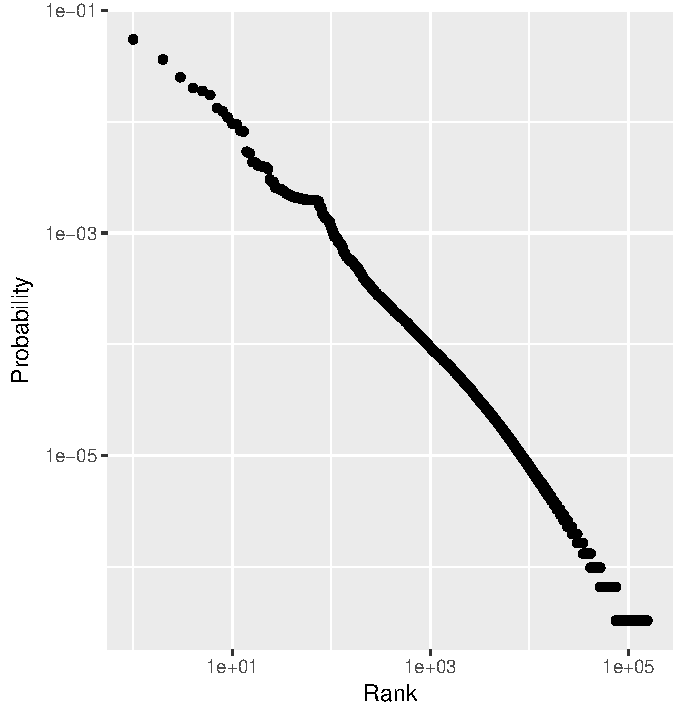
\includegraphics[scale=0.6]{unigram_plot.pdf}
  \caption{Log-log plot of unigram frequency and probability}
  \label{fig:q1p1}
  \end{figure}

   \begin{figure}[h]
  \centering
  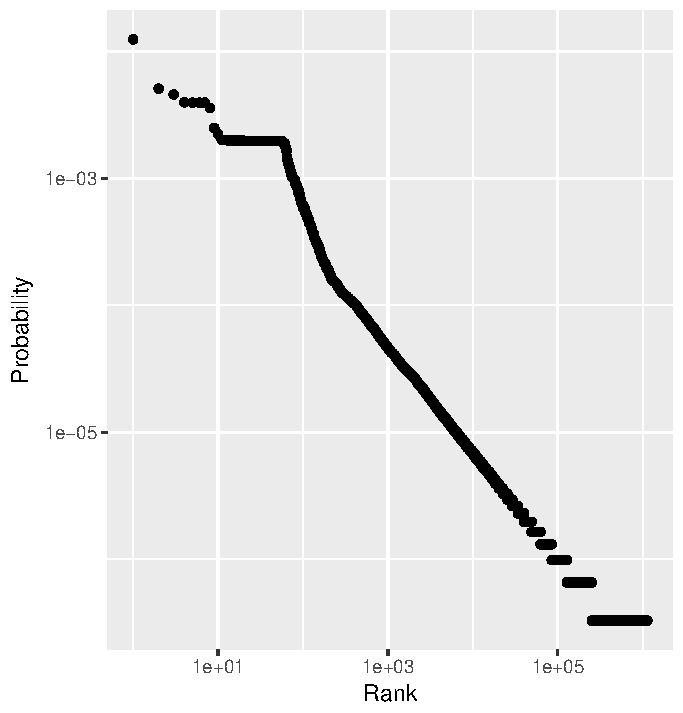
\includegraphics[scale=0.6]{bigram.pdf}
  \caption{Log-log plot of bigram frequency and probability}
  \label{fig:q1p2}
  \end{figure}
  
   \begin{figure}[h]
  \centering
  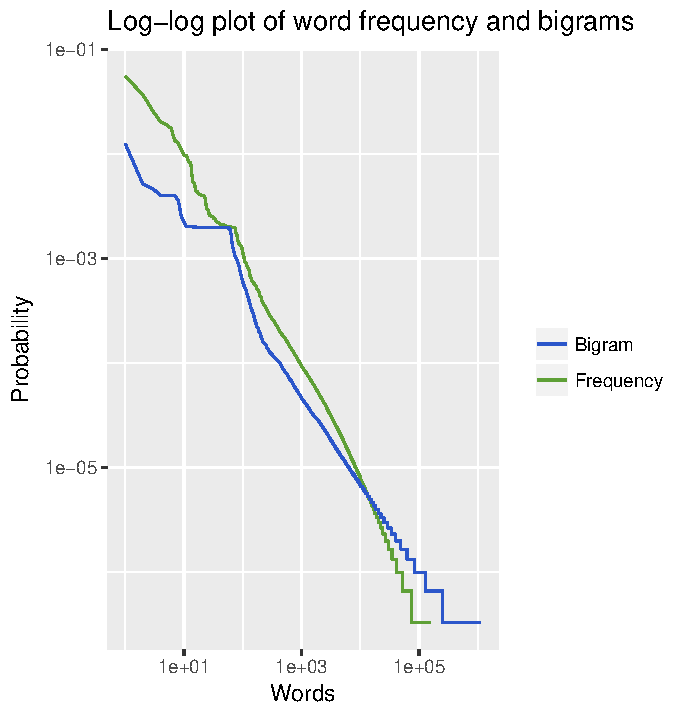
\includegraphics[scale=0.9]{unigram_and_bigram.pdf}
  \caption{Log-log plot of unigram and bigram frequencies and probabilities}
  \label{fig:q1p3}
  \end{figure}


\clearpage

% =================================
% Second question
% =================================

\section*{2}

\subsection*{Question}

\begin{verbatim}
1.4 	List five web services or sites that you use that appear to use search,
not including web search engines. Describe the role of search for that
service. Also describe the search is based on a database or grep style
of matching, or if the search is using some type of ranking.
\end{verbatim}

\subsection*{Answer}


\clearpage

% =================================
% 3rd question
% =================================

\section*{3}

\subsection*{Question}

\begin{verbatim}
3.7 	Write a program that can create a valid sitemap based on the
contents of a directory on your computer's hard disk. Assume
the file are accessible from a website at the URL http://example.com.
For instance, if there is a file in your directory called homework.pdf,
this would be available at http://www.example.com/homework.pdf.
Use the real modification date on the file as the last modified time in the
sitemap, and to help estimate the change frequency.
\end{verbatim}

\subsection*{Answer}



\clearpage

% =================================
% 4th question
% =================================

\section*{4}

\subsection*{Question}

\begin{verbatim}
Suppose that, in an effort to crawl web pages faster, you set up
two crawling machines with different starting seed URIs. Is this
an effective strategy for distributed crawling? Why or why not.
\end{verbatim}

\subsection*{Answer}


\clearpage

% =================================
% 5th question
% =================================

\section*{5}

\subsection*{Question}

\begin{verbatim}
3.9 	Write a simple single-threaded web crawler. Starting from a single input
URL (perhaps a professor's web page), the crawler should download a
page and then wait at least five seconds before downloading the next
page. Your program should find other pages to crawl by parsing link
tags found in previously crawled documents.
\end{verbatim}

\subsection*{Answer}


\clearpage


% =================================
% Bibliography
% =================================

\begin{thebibliography}{9}
\bibitem{cs532}
Atkins, Grant. ``CS532 Assignment 1 Repository'' Github. N.p., 23 March 2017. Web. 23 March 2017.\url{https://github.com/grantat/cs532-s17/tree/master/assignments/A1/src}.
\bibitem{github}
Atkins, Grant. ``CS734 Assignment 2 Repository'' Github. N.p., 21 September 2017. Web. 21 September 2017.\url{https://github.com/grantat/cs834-f17/tree/master/assignments/A2}.
\end{thebibliography}

\end{document}
